\begin{frame}{Toy Problem}
  For this implementation, we look to solve the following toy problem:

  Find $\tilde{u}\in \mathcal{R}^3$ s.t.
  \begin{equation}
    \label{eq:poisson}
    -\nabla^2 \tilde{u}+\mathbf{c}\cdot\nabla\tilde{u}+\tilde{u}=f(x,y,z),\quad \tilde{u}\in \Omega,\quad u\in\partial \Omega=0.
  \end{equation}
  for $x,y,z\in [0,1]^3$.
  We additionally choose the following manufactured solution:
  \begin{equation}
    \label{eq:mms}
    \tilde{u}=\sin\left(4\pi x\right)\sin\left(2\pi y\right)\sin\left(3\pi z\right),\quad k\in \mathcal{R}^+
  \end{equation}
  and the velocity vector $\mathbf{c}=c(1,1,1),\quad c \in \mathbb{R}, c>0$.
  This sets the forcing function to be:
  \begin{multline}
    \label{eq:mms-forcing}
    f(x,y,z)=(-29\pi^2+4\pi\cot(4\pi x)+2\pi\cot (2\pi y)+\\+3\pi\cot (3\pi z)+1)\tilde{u}(x,y,z)
  \end{multline}
\end{frame}

\begin{frame}{MMS Plot}
  \centering
  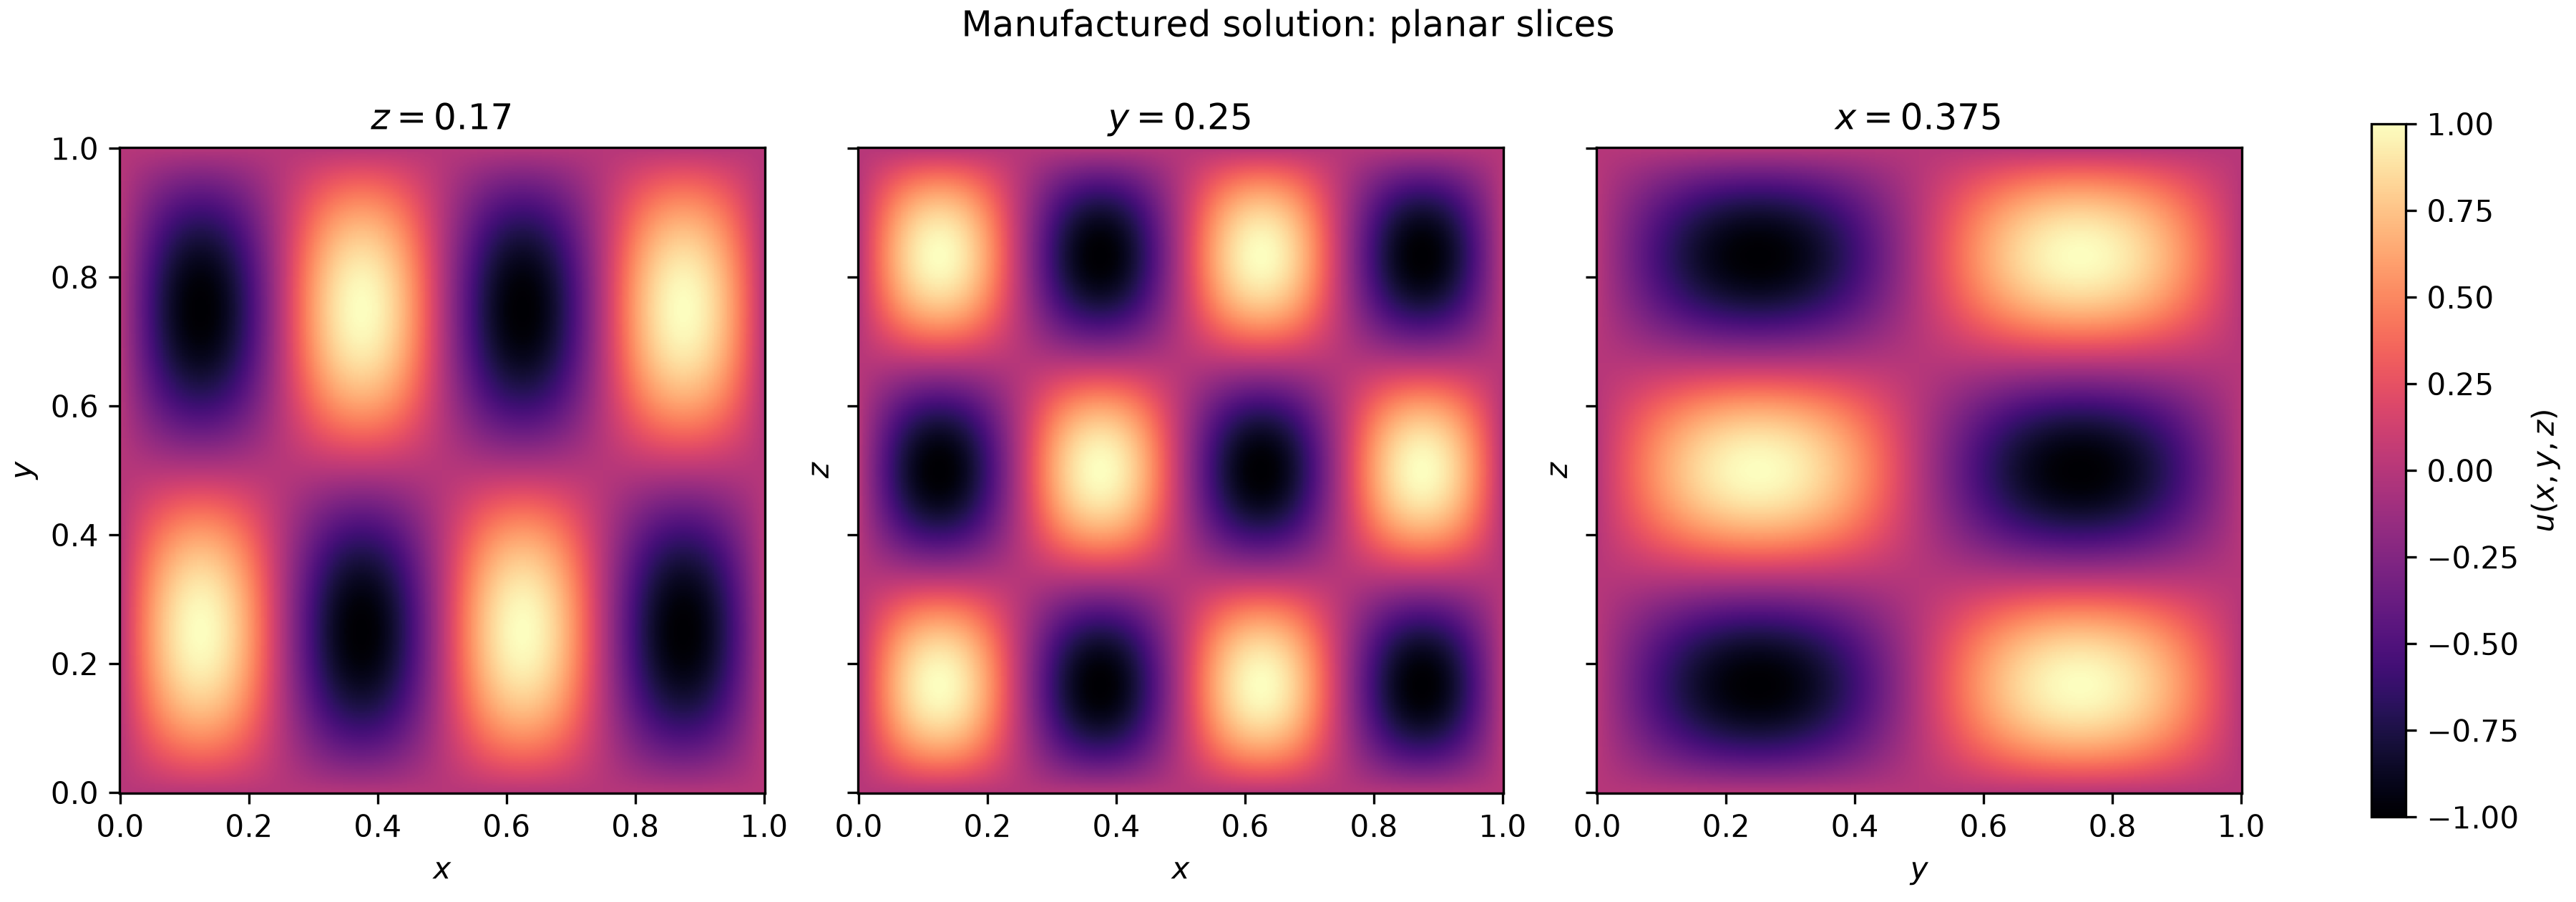
\includegraphics[width=1.05\textwidth]{figures/mms.png}
\end{frame}